\chapter{Pesos e Centro de Gravidade}
Este capítulo é a única entrada de pesos e de posição do centro de gravidade do projeto. Os valores definidos aqui (Tabela~\ref{tab:cg_entradas}) são os que devem ser usados nos capítulos de Desempenho, Cargas, Dimensionamento Estrutural e Estabilidade, que vêm depois. O capítulo segue a sequência: estimativa de pesos e fechamento no peso máximo de decolagem; posição de cada item em relação ao datum; passeio e envelope do CG, com a verificação simplificada da margem estática; e verificação preliminar da posição do trem de pouso. A verificação completa de estabilidade, estática e dinâmica, é feita no Capítulo~\ref{estabilidade} com o envelope definido aqui.

\section{Estimativa de Pesos}
A fim de determinar o peso de cada componente da aeronave, é utilizada a metodologia apresentada em Roskam, 1985, aplicada à Classe II, Commercial Transports, Regional Turboprops, acima de 12500 lbs. As equações aqui referenciadas foram retiradas do livro em questão. Para isso, são utilizados os seguintes parâmetros de entrada, que foram obtidos, majoritariamente, da análise comparativa e da definição de requisitos:

\begin{table}[H]
  \centering
  \linespread{1}\small
  \setlength{\tabcolsep}{4pt}
  \caption{Parâmetros de Pesos e Fatores de Carga}
  \label{tab:pesos_cargas}
  \begin{tabularx}{\textwidth}{c >{\raggedright\arraybackslash}X c}
    \toprule
    \textbf{Parâmetro} & \textbf{Descrição} & \textbf{Valor} \\
    \midrule
    $W_{TO}$ & Peso Máximo de Decolagem & 50.000 lb \\
    $W_{L}$ & Peso Máximo de Pouso & 49.273 lb \\
    $W_{F,max}$ & Capacidade de Combustível (sistema de combustível) & 11.000 lb \\
    $W_{MZF}$ & Peso Máximo Zero Combustível (iterado, Seção~\ref{sec:cg_pesovazio}) & 43.193 lb \\
    $n_{ult}$ & Fator de Carga Última (Manobra) & 3,75 \\
    $n_{lim}$ & Fator de Carga Limite (Manobra) & 2,5 \\
    $n_{ult,l}$ & Fator de Carga Última de Pouso & 4,0 \\
    \bottomrule
  \end{tabularx}
\end{table}

\begin{table}[H]
  \centering
  \linespread{1}\small
  \setlength{\tabcolsep}{4pt}
  \caption{Parâmetros Geométricos e de Desempenho}
  \label{tab:geometricos_desempenho}
  \begin{tabularx}{\textwidth}{c >{\raggedright\arraybackslash}X c}
    \toprule
    \textbf{Parâmetro} & \textbf{Descrição} & \textbf{Valor} \\
    \midrule
    $S$ & Área Alar & 797,6 $ft^2$ \\
    $b$ & Envergadura & 93,5 ft \\
    $A$ & Aspect Ratio & 10,96 \\
    $t_r$ & Espessura Máxima da Raiz da Asa & 2,185 ft \\
    $\Lambda_{1/2}$ & Enflechamento de Meia Corda & 0 \\
    $l_f$ & Comprimento da Fuselagem & 85,3 ft \\
    $w_f + h_f$ & Largura + Altura da Fuselagem & 18,18 ft \\
    $V_D$ & Velocidade de Mergulho de Projeto & 250 kt \\
    $V_C$ & Velocidade de Cruzeiro de Projeto & 178,6 kt \\
    \bottomrule
  \end{tabularx}
\end{table}

\subsection{Peso Estrutural}
\paragraph{Asas ($W_w$)}

Utiliza-se o método de Torenbeek para aviões de transporte (Eq. 5.7), a qual pode ser vista na \autoref{eq:W_w}.

\begin{equation}
\label{eq:W_w}
\small
W_w = 0,0017 \, W_{MZF} \left( \frac{b}{\cos \Lambda_{1/2}} \right)^{0,75}
\left[ 1 + \left( \frac{6,3 \cos \Lambda_{1/2}}{b} \right)^{1/2} \right]
n_{ult}^{0,55}
\left( \frac{bS}{t_r W_{MZF} \cos \Lambda_{1/2}} \right)^{0,30}
\end{equation}

Sendo que $W_{MZF}$ é o peso máximo zero combustível com a cabine cheia, obtido por iteração na Seção~\ref{sec:cg_pesovazio}.

O peso obtido pela Equação~\ref{eq:W_w} corresponde a uma asa de referência e é corrigido conforme a configuração, de acordo com Torenbeek: $+2\%$ pelos flaps do tipo Fowler, cujos trilhos e atuadores acrescentam massa; $+2\%$ pelos spoilers; $-5\%$ pelos motores montados na asa, cujo peso alivia o momento fletor na raiz em voo; e $-5\%$ pelo trem de pouso principal montado na fuselagem, que dispensa reforços na asa para as cargas de pouso.

\paragraph{Empenagens ($W_h$, $W_v$)}

Para aeronaves com $V_D > 250$ kt, utilizam-se as Equações 5.19 (horizontal) e 5.20 (vertical).
\subparagraph{Estabilizador Horizontal}

Com $K_h = 1,0$, para estabilizador horizontal fixo.

\begin{equation}
W_h = K_h S_h \left[
\frac{3,81 \left( S_h^{0,2} V_D \right)}{1000 \sqrt{\cos \Lambda_{1/2}}}
- 0,287
\right]
\end{equation}

\subparagraph{Estabilizador Vertical}

Com $K_v = 1 + 0,15 \frac{S_h z_h}{S_v b_v}$, para cauda em T.

\begin{equation}
W_v = K_v S_v \left[
\frac{3,81 \left( S_v^{0,2} V_D \right)}{1000 \sqrt{\cos \Lambda_{1/2}}}
- 0,287
\right]
\end{equation}


\paragraph{Fuselagem ($W_f$)}

Peso estimado pela Equação 5.27 de Torenbeek, considerando fuselagem pressurizada, tem-se o $K_f = 1,08$.

\begin{equation}
W_f = 0,021 \, K_f \sqrt{\frac{V_D \, l_h}{w_f + h_f}} \, (S_{fgs})^{1,2}
\end{equation}


\paragraph{Nacelle ($W_n$)}

Para motores turboélice, o peso das nacelles é calculado pela Equação 5.33 de Roskam:

\begin{equation}
W_n = 0,14 \cdot P_{TO,total}
\end{equation}

Onde $P_{TO,total}$ é a potência total de decolagem em shp.


\paragraph{Trem de Pouso ($W_g$)}

Calculado pela Equação 5.42, com fator de asa alta, sendo $K_{gr} = 1,08$.

\begin{equation}
W_g = K_{gr} \left[
A_g + B_g W_{TO}^{3/4} + C_g W_{TO} + D_g W_{TO}^{3/2}
\right]
\end{equation}

\begin{table}[H]
  \centering
  \linespread{1}\small
  \setlength{\tabcolsep}{4pt}
  \caption{Constantes de Torenbeek para Trem de Pouso Retrátil na fuselagem}
  \label{tab:peso_trem_constantes}
  \begin{tabularx}{\textwidth}{>{\raggedright\arraybackslash}X c c c c}
    \toprule
    \textbf{Componente} & $A_g$ & $B_g$ & $C_g$ & $D_g$ \\
    \midrule
    \textbf{Principal (Main)} & 40,0 & 0,16 & 0,019 & $1,5 \times 10^{-5}$ \\
    \textbf{Nariz (Nose)} & 20,0 & 0,10 & 0,000 & $2,0 \times 10^{-6}$ \\
    \bottomrule
  \end{tabularx}
\end{table}

\subsection{Grupo Moto-Propulsor e Acessórios}

\paragraph{Motores}

Os motores a serem utilizados são o PW127M, cujo peso seco é 1060 lbs. (480,8 kg) para cada motor, conforme 05-10-00 Manual Part No. 3037332, Revision No. 51.0.

\paragraph{Sistema de Combustível}

Equação 6.24 para tanques integrais:

\begin{equation}
W_{fs} = 80(N_e + N_t - 1) + 15\sqrt{N_t} (W_F / K_{fsp})^{0,333}
\end{equation}

Em que, $K_{fsp}$ é a densidade do combustível QAV em lbs/gal.


\paragraph{Hélice}

De acordo com o manual de treinamento da Caribbean Airlines, o avião é equipado com duas hélices, e cada um desses sistemas pesa cerca de 159 kg (350 libras).

Essa hélice previamente escolhida foi a HAMILTON STANDARD 568F, que equipa as aeronaves ATR72-600.

\paragraph{Controladores}

Equação 6.25 para turbopropulsores na asa:

\begin{equation}
W_{ec} = 56,84 \left[ \frac{(l_f + b) N_e}{100} \right]^{0,514}
\end{equation}

\paragraph{Sistema de Partida}

Equação 6.30 para sistemas pneumáticos:

\begin{equation}
W_{ess} = 12,05 (W_{e,total} / 1.000)^{1,458}
\end{equation}


\subsection{Equipamentos Fixos}

\paragraph{Controles de Voo}

Calculado pela Equação 7.6 para aeronaves com controles de voo assistidos:

\begin{equation}
    W_{fc} = K_{fc} (W_{TO})^{2/3}
\end{equation}

onde $K_{fc} = 0,64$.

\paragraph{Sistema Hidráulico e Pneumático}

Conforme a metodologia adotada, o peso do sistema hidráulico e/ou pneumático necessário para os controles de voo assistidos já foi computado na previsão de peso do sistema de controle de voo.

\paragraph{Sistema Elétrico}

Estimado pela Equação 7.16:

\begin{equation}
    W_{els} = 0,325 (W_E)^{0,8}
\end{equation}

\paragraph{Aviônicos e Instrumentação}

Estimado inicialmente pela Equação 7.24:

\begin{equation}
    W_{iae} = 120 + 20N_e + 0,006W_{TO}
\end{equation}

A equação original é provavelmente muito conservadora, já que os sistemas aviônicos atuais são significativamente mais leves do que aqueles existentes quando a equação foi determinada. Para efeito de comparação, a Thales, fabricante dos aviônicos do ATR72, afirma que o Integrated Modular Avionics (IMA) reduz em até 40\% o peso do sistema. Esse valor foi considerado para redução do peso estimado.

\paragraph{Sistema de Pressurização e Ar-condicionado}

Para aeronaves pressurizadas, utiliza-se a Equação 7.30, baseada no comprimento da cabine de passageiros ($l_{pax}$):

\begin{equation}
    W_{api} = 6,75 (l_{pax})^{1,28}
\end{equation}

\paragraph{Sistema de Oxigênio}

Calculado pela Equação 7.36 para voos abaixo de 25.000 ft:

\begin{equation}
    W_{ox} = 20 + 0,5N_{pax}
\end{equation}


\paragraph{Mobiliário}

Peso do mobiliário interno estimado pela Equação 7.45:

\begin{equation}
    W_{fur} = 0,211 (W_{TO} - W_F)^{0,91}
\end{equation}

em que $W_{TO} - W_F$ é o peso zero combustível, tomado igual ao $W_{MZF}$ iterado na Seção~\ref{sec:cg_pesovazio}.

\paragraph{Equipamento para acomodação de carga e bagagem}

Estimado pela Equação 7.49, baseada na área do piso de carga ($S_{ff}$):

\begin{equation}
    W_{bc} = 3 S_{ff}
\end{equation}

\paragraph{Tinta}

Peso estimado pela Equação 7.51:

\begin{equation}
    W_{pt} = 0,003 W_{TO}
\end{equation}

\subsection{Resultados das Estimativas de Peso}
\begin{table}[H]
  \centering
  \linespread{1}\small
  \setlength{\tabcolsep}{4pt}
  \caption{Estimativa do peso vazio por componente (Classe II), com $W_{MZF}$ iterado.}
  \label{tab:oew_componentes}
  \begin{tabularx}{\textwidth}{>{\raggedright\arraybackslash}X r r}
    \toprule
    \textbf{Componente} & \textbf{Peso (lb)} & \textbf{Peso (kg)} \\
    \midrule
    \multicolumn{3}{l}{\textit{Grupo Estrutural}} \\
    Peso da Asa & 5033,82 & 2283,28 \\
    Estabilizador Horizontal & 495,46 & 224,74 \\
    Estabilizador Vertical & 464,60 & 210,74 \\
    Fuselagem & 8163,47 & 3702,88 \\
    Nacelle & 770,00 & 349,27 \\
    Trem de Pouso Principal & 1828,11 & 829,22 \\
    Trem de Pouso de Nariz & 406,87 & 184,55 \\
    \addlinespace
    \multicolumn{3}{l}{\textit{Grupo Moto-Propulsor}} \\
    Motores (PW127M) & 2120,00 & 961,62 \\
    Hélices & 700,00 & 317,51 \\
    Acessórios de Instalação & 127,20 & 57,70 \\
    Sistema de Combustível & 491,53 & 222,95 \\
    Controles do Motor (Wec) & 109,42 & 49,63 \\
    Sistema de Partida (Wess) & 36,04 & 16,35 \\
    \addlinespace
    \multicolumn{3}{l}{\textit{Grupo de Equipamentos Fixos}} \\
    Controles de Voo & 868,61 & 394,00 \\
    Aviônicos (IMA) & 276,00 & 125,19 \\
    Sistema Elétrico & 1500,00 & 680,39 \\
    Ar-cond./Pressurização/Degelo & 1356,62 & 615,35 \\
    Sistema de Oxigênio & 56,00 & 25,40 \\
    Mobiliário/Furnishings & 3487,48 & 1581,87 \\
    Equipamento de Carga/Bagagem & 360,00 & 163,29 \\
    Tinta & 150,00 & 68,04 \\
    \midrule
    \textbf{Peso vazio ($W_E$)} & \textbf{28801,24} & \textbf{13063,97} \\
    \bottomrule
  \end{tabularx}
\end{table}

\subsection{Peso vazio}
\label{sec:cg_pesovazio}
O peso vazio ($W_E$) é o somatório dos grupos estrutural, motopropulsor e de equipamentos fixos, estimados pelo método Classe~II nas seções anteriores. Duas dessas correlações dependem do peso zero combustível: a da asa, proporcional a $W_{MZF}^{0,70}$, e a do mobiliário, proporcional a $(W_{TO}-W_F)^{0,91}$, em que $W_{TO}-W_F$ é o próprio peso zero combustível. Na primeira avaliação, essas equações foram feitas com $W_F = 11\,000$ lb, que é a capacidade dos tanques, o que equivale a supor decolagem no MTOW com tanques cheios. Com 64 passageiros essa hipótese não se sustenta (Seção~\ref{sec:cg_fechamento}), e o valor de projeto passa a ser o MZFW da cabine cheia. Como o MZFW depende do peso vazio, as duas correlações são iteradas até a convergência:

\begin{equation}
W_{MZF}^{(k+1)} = W_E\!\left(W_{MZF}^{(k)}\right) + W_{trip} + W_{cat} + W_{CP},
\label{eq:cg_iteracao}
\end{equation}
em que $W_{trip}$ é a tripulação, $W_{cat}$ o catering e $W_{CP}$ a carga paga. A iteração converge em poucos passos e altera apenas dois itens: a asa, de 2\,125,8 para 2\,283,3 kgf, e o mobiliário, de 1\,441,5 para 1\,581,9 kgf. A Tabela~\ref{tab:oew_componentes} já apresenta os valores convergidos. Os demais itens não mudam, porque dependem do MTOW (fixo) ou da capacidade de combustível (fixa). O peso vazio resulta em $W_E = 13\,064$ kgf.

\subsection{Tripulação, passageiros e bagagem}
Adotam-se as massas-padrão da regulamentação de operações da EASA \cite{easa_airops}, já que o projeto usa a base normativa ANAC/FAA/EASA. Para aeronaves com 30 ou mais assentos, a norma admite 84 kg por passageiro adulto, com bagagem de mão incluída, e 11 kg por volume de bagagem despachada em voos domésticos. Para a tripulação, os valores são 85 kg por tripulante técnico e 75 kg por comissário, também com bagagem de mão. A Tabela~\ref{tab:cg_massas} resume os valores.

\begin{table}[H]
  \centering
  \linespread{1}\small
  \setlength{\tabcolsep}{4pt}
  \caption{Massas-padrão adotadas para pessoas e bagagem \cite{easa_airops}.}
  \label{tab:cg_massas}
  \begin{tabularx}{\textwidth}{>{\raggedright\arraybackslash}X c c c}
    \toprule
    \textbf{Item} & \textbf{Quantidade} & \textbf{Massa unitária [kgf]} & \textbf{Total [kgf]} \\
    \midrule
    Pilotos & 2 & 85 & 170 \\
    Comissários & 2 & 75 & 150 \\
    Passageiros (com bagagem de mão) & 64 & 84 & 5\,376 \\
    Bagagem despachada (doméstico) & 64 & 11 & 704 \\
    \bottomrule
  \end{tabularx}
\end{table}

\subsection{Fechamento no peso máximo de decolagem}
\label{sec:cg_fechamento}
O MTOW de 50\,000 lb (22\,680 kgf) é requisito de projeto e não é ultrapassado. Ele é composto pelo peso vazio operacional (OEW), pela carga paga e pelo combustível. O OEW inclui a tripulação e o catering, que estão a bordo em qualquer voo. Com a cabine cheia, o combustível disponível é o que falta para chegar ao MTOW:

\begin{equation}
W_{F} = MTOW - MZFW = 22\,680 - 19\,592 = 3\,088 \ \text{kgf}.
\label{eq:cg_combustivel}
\end{equation}

\begin{table}[H]
  \centering
  \linespread{1}\small
  \setlength{\tabcolsep}{4pt}
  \caption{Composição dos pesos da aeronave (configuração de passageiros).}
  \label{tab:cg_pesos}
  \begin{tabularx}{\textwidth}{>{\raggedright\arraybackslash}X r}
    \toprule
    \textbf{Parcela} & \textbf{Peso [kgf]} \\
    \midrule
    Peso vazio, $W_E$ (Classe II, iterado) & 13\,064 \\
    Tripulação (2 pilotos + 2 comissários) & 320 \\
    \emph{Catering} / \emph{galley} & 128 \\
    \textbf{Peso vazio operacional (OEW)} & \textbf{13\,512} \\
    Passageiros (64) & 5\,376 \\
    Bagagem despachada & 704 \\
    \textbf{Peso máximo zero combustível (MZFW)} & \textbf{19\,592} \\
    Combustível com carga paga máxima & 3\,088 \\
    \textbf{Peso máximo de decolagem (MTOW)} & \textbf{22\,680} \\
    \bottomrule
  \end{tabularx}
\end{table}

A capacidade dos tanques continua sendo de 4\,990 kgf. Ela só pode ser usada inteira com carga paga reduzida, como em qualquer aeronave de transporte. A Tabela~\ref{tab:cg_cargapaga} mostra os dois pontos que limitam o diagrama carga paga--alcance.


\begin{table}[H]
  \centering
  \linespread{1}\small
  \setlength{\tabcolsep}{4pt}
  \caption{Pontos limite de carga paga e combustível no MTOW.}
  \label{tab:cg_cargapaga}
  \begin{tabularx}{\textwidth}{>{\raggedright\arraybackslash}X c c c}
    \toprule
    \textbf{Condição} & \textbf{Carga paga [kgf]} & \textbf{Combustível [kgf]} & \textbf{Limitada por} \\
    \midrule
    Carga paga máxima & 6\,080 & 3\,088 & MZFW e MTOW \\
    Combustível máximo & 4\,178 & 4\,990 & Tanques e MTOW \\
    \bottomrule
  \end{tabularx}
\end{table}

O ATR~72-600, de MTOW e grupo motopropulsor semelhantes, serve de verificação de ordem de grandeza \cite{atr72600}, com OEW típico em serviço de 13\,600 kg, contra 13\,512 kgf aqui. Com MTOW de 23\,000 kg e 70 passageiros de 95 kg, seu alcance com passageiros máximos é de 740 NM, com reservas EASA e alternativa a 100 NM, o que corresponde a cerca de 2\,750 kg de combustível. Os 3\,088 kgf disponíveis aqui, para 800 NM com 64 passageiros, estão na mesma ordem de grandeza. O peso máximo de pouso de 22\,350 kgf é respeitado em qualquer pouso realizado após o consumo de mais de 330 kgf de combustível.

\section{Datum e Posição dos Itens}
\label{sec:cg_posicoes}
O datum é a ponta do nariz da fuselagem, com o eixo $x$ positivo em direção à cauda. É o mesmo referencial dos desenhos. A Figura~\ref{fig:cg_esquema} mostra a posição de todos os itens de peso sobre a vista lateral, com o datum, a CMA e a faixa de CG admissível. A numeração da figura é a da Tabela~\ref{tab:cg_bracos}.


\begin{figure}[H]
\centering
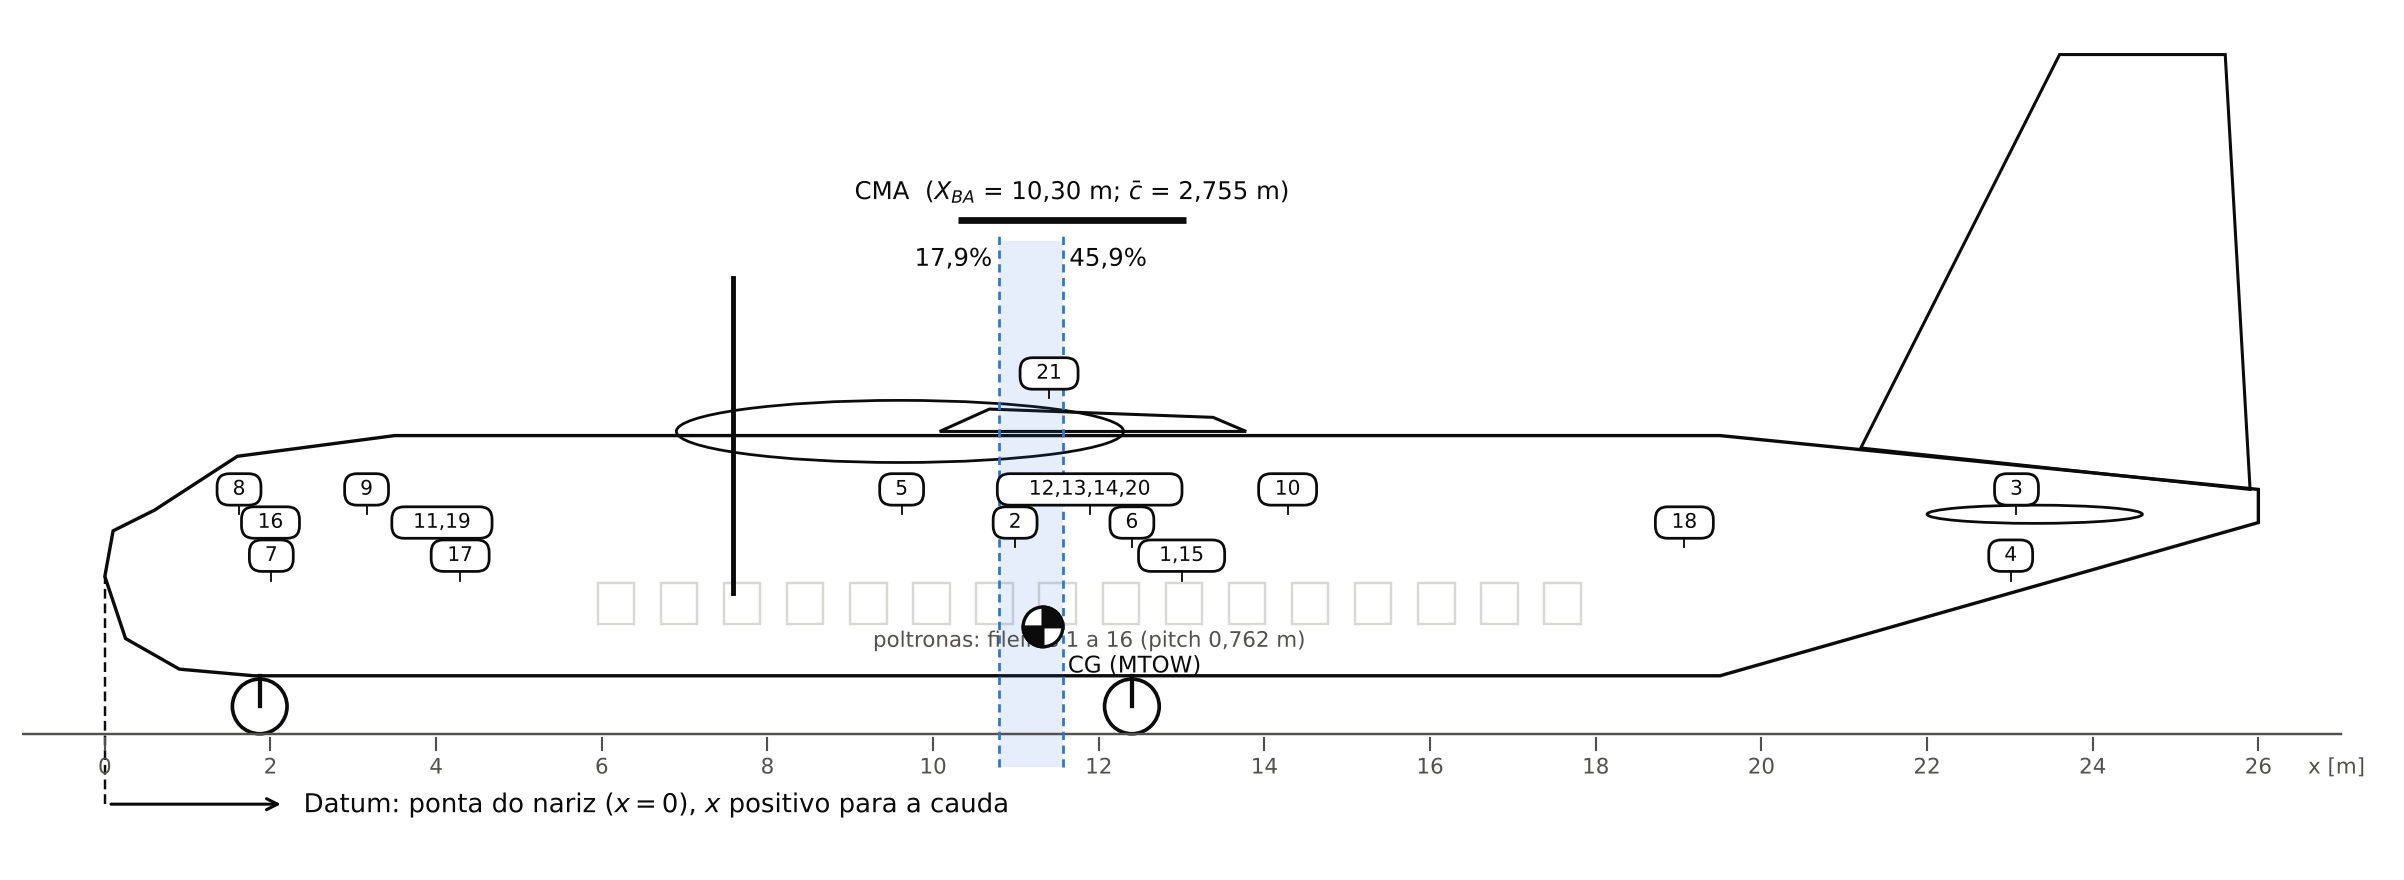
\includegraphics[width=\textwidth]{Images-CG/cg_esquema_lateral.png}
\caption{Diagrama esquemático da vista lateral com a posição dos itens de peso, o datum, a CMA e a faixa de CG admissível.}
\label{fig:cg_esquema}
\end{figure}

\begin{figure}[H]
\centering
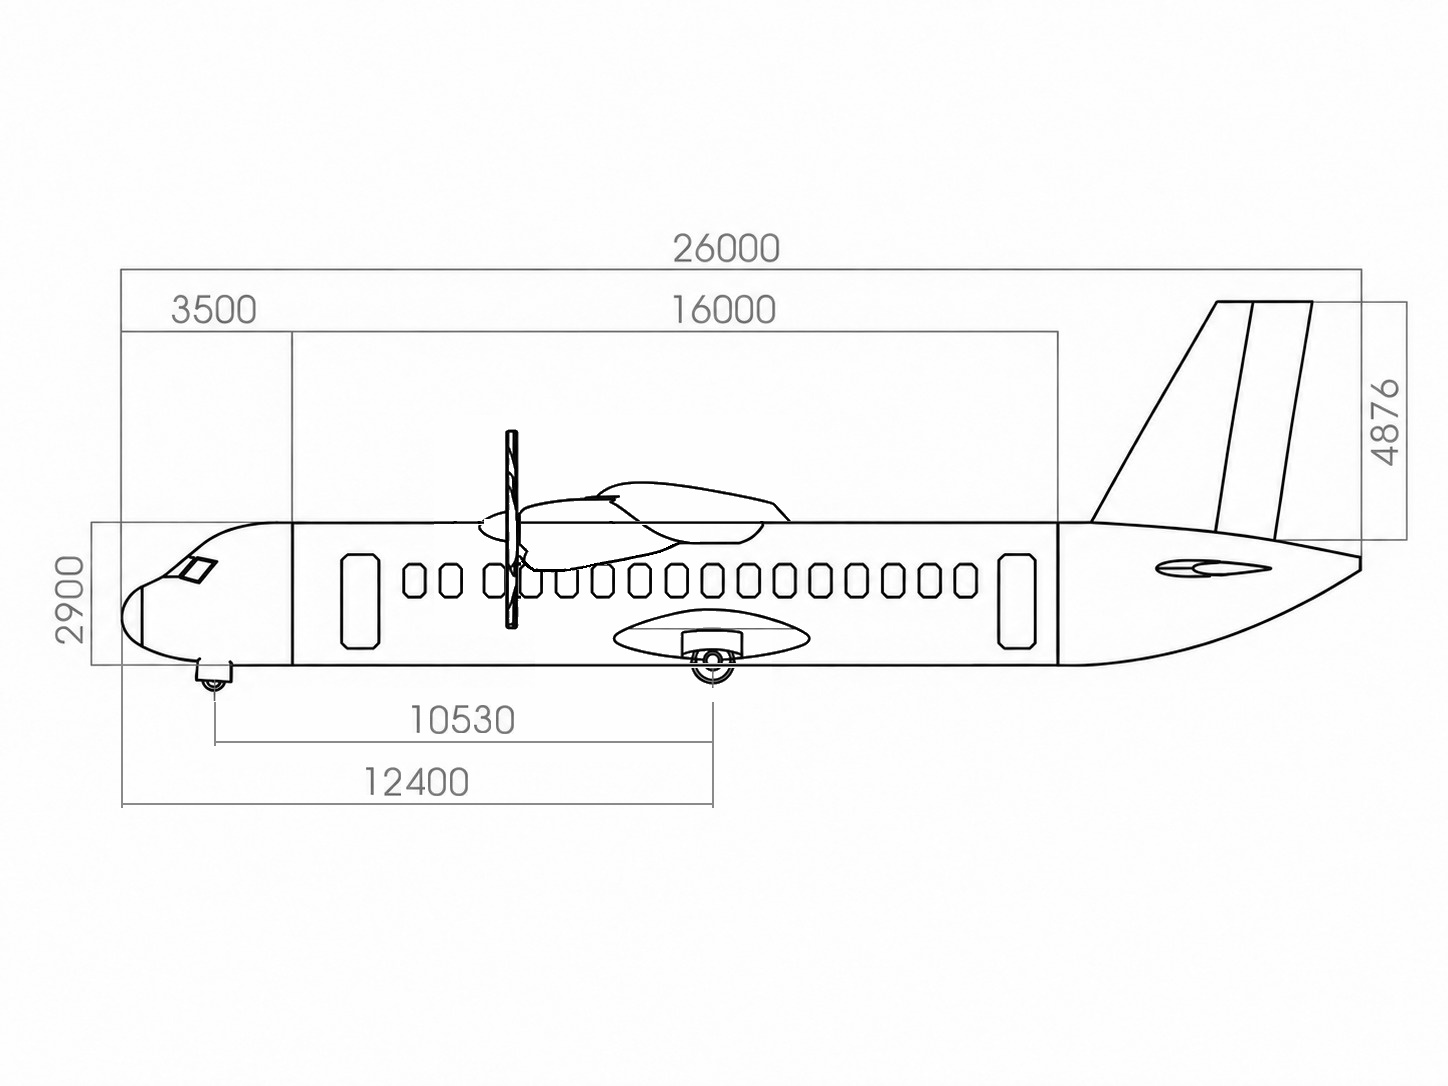
\includegraphics[width=0.85\textwidth]{Images-CG/VistaLateral.jpeg}
\caption{Vista lateral com cotas usada como referência geométrica.}
\label{fig:cg_vista_ref}
\end{figure}

\subsection{Posição da asa}

A posição da asa é definida pelo bordo de ataque da CMA, $X_{BA,\text{CMA}} = 10{,}30$ m, com $\bar{c} = 2{,}755$ m. Essa é a posição em que o braço da empenagem horizontal ($l_{EH} = 12{,}0$ m) e o volume de cauda ($\bar{V}_{HT} = 1{,}1$) da Conclusão do Anteprojeto (Tabela~\ref{tab:dimensoes_conclusao}) são consistentes: o centro aerodinâmico da asa fica em 10,99 m e o da empenagem em 22,99 m, junto ao braço de 23,08 m da empenagem horizontal.

Os itens presos à asa acompanham sua posição. O O CG da asa mantém a posição relativa adotada no anteprojeto, a 25\% da CMA (0,686 m atrás do bordo de ataque) O combustível, nos tanques integrais, é posicionado a 40\% da CMA (11,40 m).

O braço do grupo motopropulsor foi estimado pelos seus subcomponentes, com as distâncias ao bordo de ataque da CMA medidas na vista lateral (Tabela~\ref{tab:cg_gmp}). O resultado coloca o conjunto 0,68 m à frente do bordo de ataque da CMA, coerente com motores montados à frente da asa.

\begin{table}[H]
  \centering
  \linespread{1}\small
  \setlength{\tabcolsep}{4pt}
  \caption{Estimativa do braço do grupo motopropulsor por subcomponentes (distâncias ao bordo de ataque da CMA).}
  \label{tab:cg_gmp}
  \begin{tabularx}{\textwidth}{>{\raggedright\arraybackslash}X c c c}
    \toprule
    \textbf{Subcomponente} & \textbf{Peso [kgf]} & \textbf{Distância ao BA da CMA [m]} & \textbf{Referência} \\
    \midrule
    Hélices (2) & 317,5 & $-2{,}14$ & Plano do disco \\
    Motores PW127M (2) & 961,6 & $-1{,}02$ & Centro do motor \\
    Acessórios, controles e partida & 123,7 & $-1{,}02$ & Junto ao motor \\
    Naceles & 349,3 & $+0{,}58$ & Centroide da nacele \\
    Sistema de combustível & 223,0 & $+1{,}10$ & 40\% da CMA \\
    \midrule
    \textbf{Grupo motopropulsor} & \textbf{1\,975,0} & $\mathbf{-0{,}68}$ & $x = 9{,}62$ m \\
    \bottomrule
  \end{tabularx}
\end{table}

\subsection{Itens fixos à fuselagem}

As empenagens e o trem de nariz têm braço obtido da geometria do desenho. A fuselagem é posicionada a 50\% do seu comprimento (13,00 m), hipótese usual para uma estrutura de seção aproximadamente constante. Comandos de voo, aviônicos, equipamento de carga e o sistema de ar-condicionado e pressurização são posicionados conforme o arranjo interno: os comandos no posto de pilotagem (1,62 m), os aviônicos na baia logo atrás da cabine de comando (3,16 m), o equipamento de carga no compartimento de bagagem dianteiro (4,07 m) e os packs de ar-condicionado em um compartimento ventral não pressurizado logo atrás da raiz da asa (14,28 m), como em aeronaves da mesma classe. O item de ar-condicionado da Classe~II de Roskam engloba também a proteção contra gelo, de modo que os 120 kgf do sistema de degelo estão contidos nos 615,4 kgf desse item. Os sistemas elétrico e de oxigênio e o mobiliário, que se distribuem ao longo da cabine, são posicionados no centroide das 16 fileiras de passageiros (11,89 m). A tinta é posicionada no centroide da fuselagem (13,00 m).

\begin{table}[H]
  \centering
  \linespread{1}\small
  \setlength{\tabcolsep}{4pt}
  \caption{Pesos, braços e momentos do peso vazio e do peso vazio operacional ($X_{BA,\text{CMA}} = 10{,}30$ m; trem principal em 12,40 m).}
  \label{tab:cg_bracos}
  \begin{tabularx}{\textwidth}{c >{\raggedright\arraybackslash}X r r r >{\raggedright\arraybackslash}X}
    \toprule
    \textbf{N.º} & \textbf{Item} & \textbf{Peso [kgf]} & \textbf{Braço [m]} & \textbf{Momento [kgf$\cdot$m]} & \textbf{Origem do braço} \\
    \midrule
    1 & Fuselagem & 3\,702,9 & 13,00 & 48\,137 & Hipótese: 50\% de $l_f$ \\
    2 & Asa & 2\,283,3 & 10,99 & 25\,084 & 25\% da CMA \\
    3 & Empenagem horizontal & 224,7 & 23,08 & 5\,187 & Desenho \\
    4 & Empenagem vertical & 210,7 & 23,01 & 4\,849 & Desenho \\
    5 & Grupo motopropulsor & 1\,974,9 & 9,62 & 18\,999 & Tabela~\ref{tab:cg_gmp} \\
    6 & Trem de pouso principal & 829,2 & 12,40 & 10\,282 & Seção~\ref{sec:cg_trem} \\
    7 & Trem de pouso de nariz & 184,6 & 2,01 & 371 & Desenho \\
    8 & Comandos de voo & 394,0 & 1,62 & 638 & Posto de pilotagem \\
    9 & Aviônicos & 125,2 & 3,16 & 396 & Baia de aviônicos \\
    10 & Ar-cond., pressurização e degelo & 615,4 & 14,28 & 8\,787 & Compartimento ventral \\
    11 & Equip. de carga e bagagem & 163,3 & 4,07 & 665 & Compartimento dianteiro \\
    12 & Sistema elétrico & 680,4 & 11,89 & 8\,088 & Centroide da cabine \\
    13 & Sistema de oxigênio & 25,4 & 11,89 & 302 & Centroide da cabine \\
    14 & Mobiliário & 1\,581,9 & 11,89 & 18\,805 & Centroide da cabine \\
    15 & Tinta & 68,0 & 13,00 & 885 & Centroide da fuselagem \\
    \midrule
     & \textbf{Peso vazio, $W_E$} & \textbf{13\,063,9} & \textbf{11,59} & \textbf{151\,475} & \\
    \midrule
    16 & Pilotos (2 × 85 kgf) & 170,0 & 2,00 & 340 & Cabine de comando \\
    17 & Comissários (2 × 75 kgf) & 150,0 & 4,29 & 644 & Assentos de comissário \\
    18 & \emph{Catering} / \emph{galley} & 128,0 & 19,07 & 2\,441 & \emph{Galley} traseira \\
    \midrule
     & \textbf{Peso vazio operacional, OEW} & \textbf{13\,511,9} & \textbf{11,46} & \textbf{154\,900} & \\
    \midrule
    19 & Bagagem despachada & 704,0 & 4,07 & 2\,865 & Compartimento dianteiro \\
    20 & Passageiros (centroide) & 5\,376,0 & 11,89 & 63\,909 & Fileiras 1 a 16 \\
    21 & Combustível com carga paga máxima & 3\,088,0 & 11,40 & 35\,209 & 40\% da CMA \\
    \bottomrule
  \end{tabularx}
\end{table}

O CG em porcentagem da CMA é obtido por
\begin{equation}
\bar{X}_{CG} = \frac{\sum W_i x_i}{\sum W_i}, \qquad
h_{CG} = \frac{\bar{X}_{CG} - X_{BA,\text{CMA}}}{\bar{c}} \times 100\%.
\label{eq:cg}
\end{equation}

\section{Passeio e Envelope do CG}
\label{sec:cg_envelope}

\subsection{Condições de carregamento}

A partir do OEW, a carga útil é somada item a item e o CG é recalculado a cada passo. A bagagem despachada é carregada primeiro, no compartimento dianteiro. Os passageiros embarcam em grupos de quatro fileiras, em duas sequências: da frente para trás e de trás para a frente. Essas sequências limitam o passeio, já que qualquer outra ordem de embarque produz posições entre elas. As mesmas sequências são repetidas sem bagagem despachada, caso em que o CG fica mais traseiro. O combustível, a 40\% da CMA, aproxima o CG dessa posição. Por isso as condições sem combustível, que também representam o pouso com reserva mínima, são as mais extremas. A Tabela~\ref{tab:cg_passeio} e a Figura~\ref{fig:cg_envelope} apresentam os resultados.

\begin{table}[H]
  \centering
  \linespread{1}\small
  \setlength{\tabcolsep}{4pt}
  \caption{Passeio do CG por condição de carregamento ($X_{BA,\text{CMA}} = 10{,}30$ m; $\bar{c} = 2{,}755$ m).}
  \label{tab:cg_passeio}
  \begin{tabularx}{\textwidth}{>{\raggedright\arraybackslash}X c c c}
    \toprule
    \textbf{Condição} & \textbf{Peso [kgf]} & $\bar{X}_{CG}$ \textbf{[m]} & $h_{CG}$ \textbf{[\% CMA]} \\
    \midrule
    OEW & 13\,512 & 11,46 & 42,2 \\
    OEW + bagagem & 14\,216 & 11,10 & 29,0 \\
    \multicolumn{4}{l}{\textit{Embarque da frente para trás (com bagagem)}} \\
    \quad fileiras 1--4 & 15\,560 & 10,77 & 17,1 \\
    \quad fileiras 1--8 & 16\,904 & 10,74 & 15,9 \\
    \quad fileiras 1--12 & 18\,248 & 10,94 & 23,1 \\
    \multicolumn{4}{l}{\textit{Embarque de trás para a frente (com bagagem)}} \\
    \quad fileiras 13--16 & 15\,560 & 11,56 & 45,8 \\
    \quad fileiras 9--16 & 16\,904 & 11,71 & 51,1 \\
    \quad fileiras 5--16 & 18\,248 & 11,61 & 47,5 \\
    MZFW (cabine cheia, com bagagem) & 19\,592 & 11,32 & 36,8 \\
    MTOW (cabine cheia, 3\,088 kgf de combustível) & 22\,680 & 11,33 & 37,3 \\
    Cabine cheia, sem bagagem, sem combustível & 18\,888 & 11,58 & 46,6 \\
    \bottomrule
  \end{tabularx}
\end{table}

\begin{figure}[H]
\centering
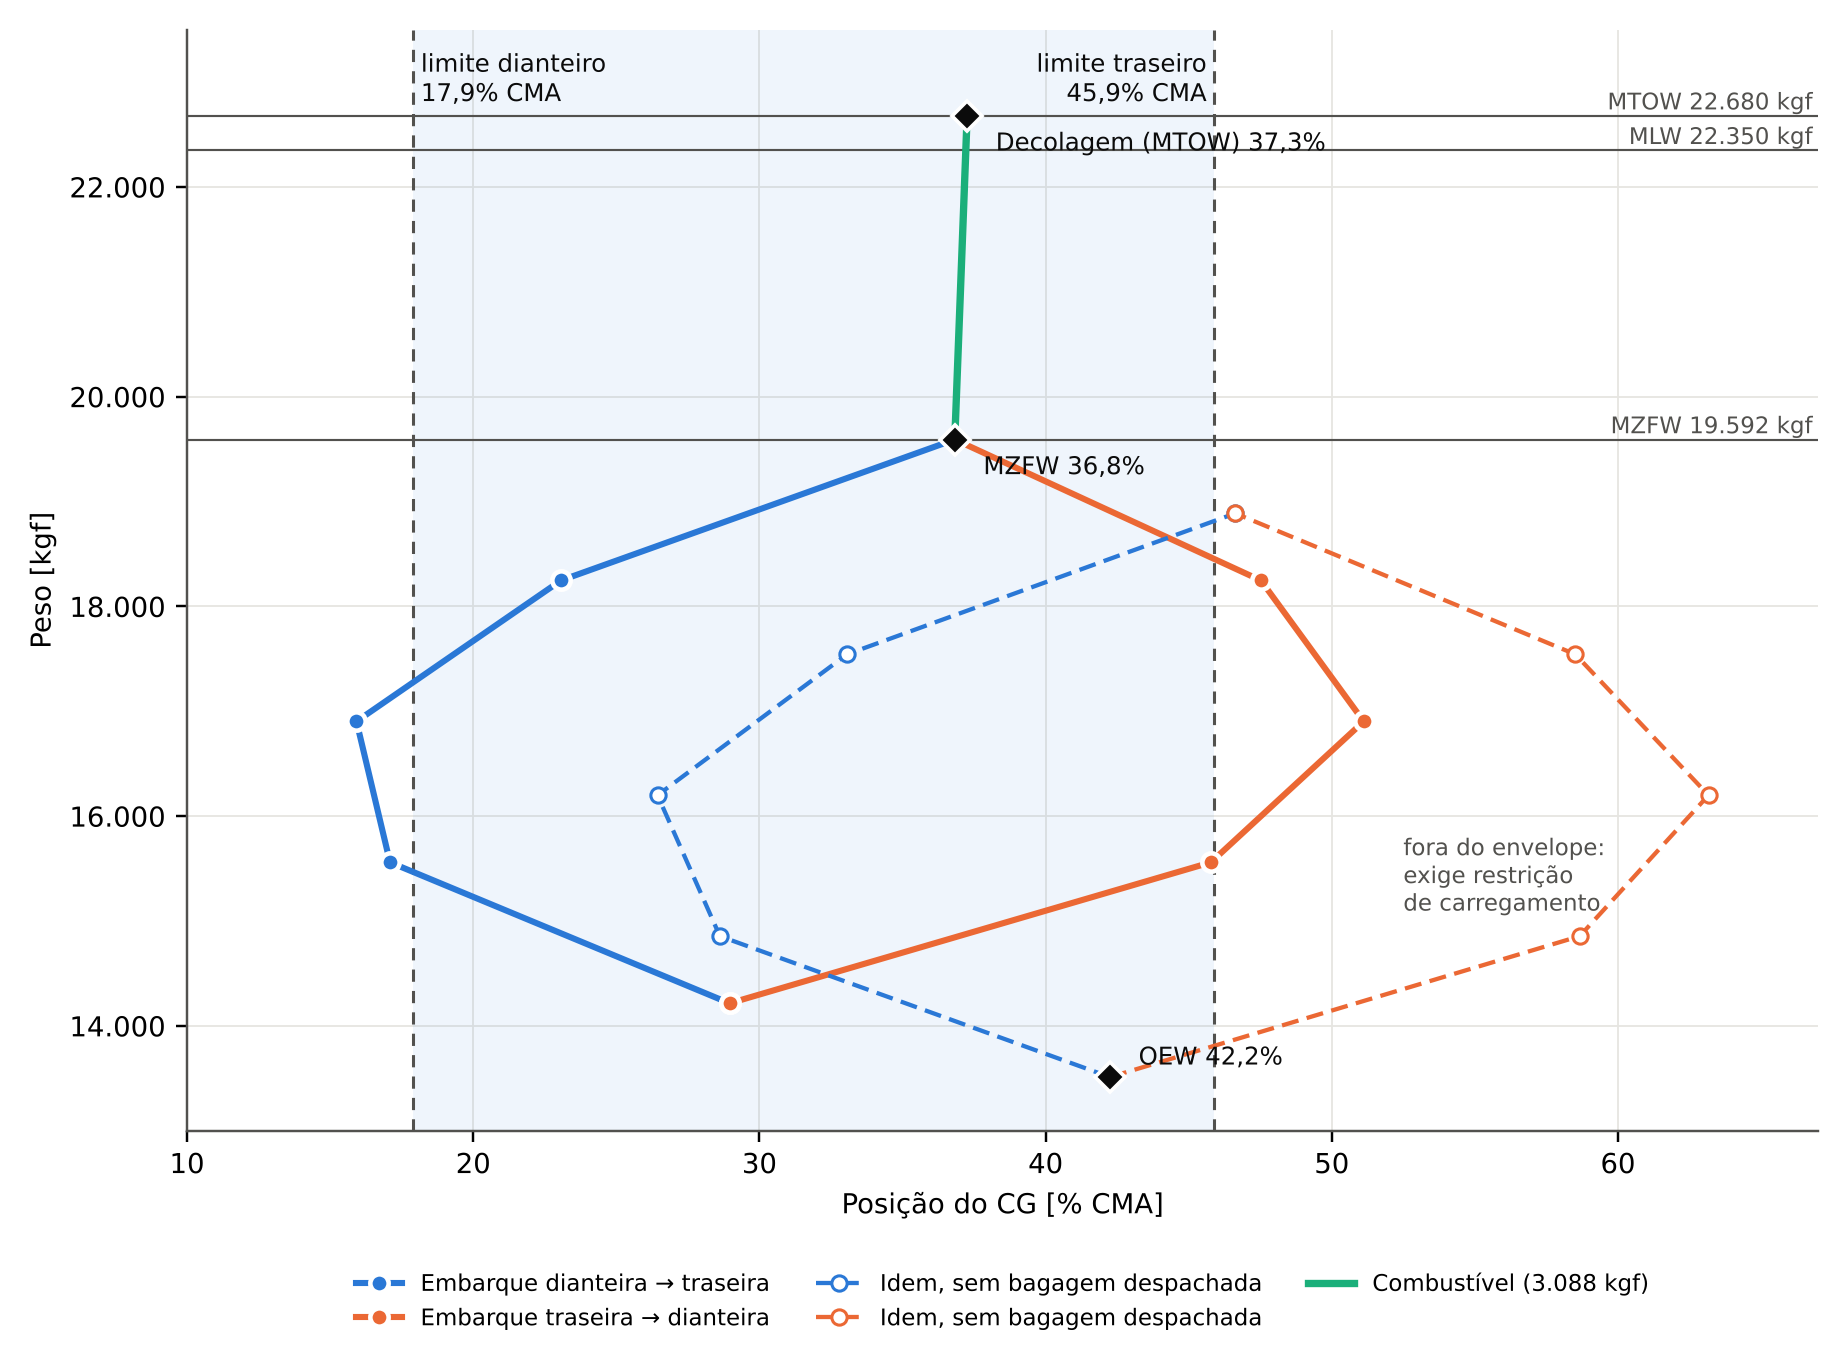
\includegraphics[width=0.92\textwidth]{Images-CG/cg_envelope.png}
\caption{Envelope de CG para o operador: limites de CG, pesos limite e linhas de carregamento. Linhas cheias com bagagem despachada; tracejadas sem bagagem despachada.}
\label{fig:cg_envelope}
\end{figure}

\subsection{Limites de CG e verificação simplificada da margem estática}
\label{sec:cg_margem}

Os limites de CG propostos são 17,9\% da CMA (dianteiro) e 45,9\% da CMA (traseiro), ou seja, $\bar{X}_{CG}$ entre 10,79 m e 11,56 m. As condições de cabine cheia (MZFW, MTOW e pouso) ficam entre 36,8\% e 37,3\% da CMA, longe dos dois limites. O OEW, a 42,2\%, também está dentro deles.

A verificação simplificada usa a margem estática $ME = h_n - h_{CG}$, com o ponto neutro estimado pela contribuição da asa e da empenagem horizontal \cite{raymer2018}:
\begin{equation}
h_n = h_{ca} + \eta_h \, \bar{V}_{HT} \, \frac{a_h}{a_w}\left(1 - \frac{d\varepsilon}{d\alpha}\right).
\label{eq:cg_ponto_neutro}
\end{equation}
Com $h_{ca} = 0{,}25$, $\eta_h = 0{,}9$, $\bar{V}_{HT} = 1{,}098$, $a_w = 5{,}24$ rad$^{-1}$ ($A = 10{,}96$), $a_h = 3{,}77$ rad$^{-1}$ ($A_h = 3{,}76$) e $d\varepsilon/d\alpha = 2a_w/(\pi A) = 0{,}30$, obtém-se $h_n = 0{,}745$. As inclinações das curvas de sustentação foram estimadas pela fórmula de Helmbold para asa sem enflechamento. O AVL, no Capítulo~\ref{estabilidade}, fornece $h_n = 0{,}766$, valor próximo deste. A margem estática resulta em 56,6\% no limite dianteiro e 28,6\% no limite traseiro, positiva em todo o envelope.

A equação~\eqref{eq:cg_ponto_neutro} não inclui o efeito desestabilizante da fuselagem, que desloca o ponto neutro para a frente. Mesmo com uma redução de 0,15$\bar{c}$ por esse efeito, a margem no limite traseiro continuaria positiva, próxima de 14\%. As margens elevadas refletem o volume de cauda de 1,1. O efeito na força de profundor na rotação e no arrasto de compensação, bem como a verificação do limite dianteiro, são tratados no Capítulo~\ref{estabilidade}.

\textbf{Precisa deslocar a asa?} Não, além do deslocamento de 0,58 m para trás já adotado. Na posição do anteprojeto e do desenho atual ($X_{BA,\text{CMA}} = 9{,}72$ m), com os braços corrigidos, o OEW ficaria a 56,7\% da CMA, o MZFW a 53,3\% e o carregamento mais traseiro a 78,7\%, praticamente sobre o ponto neutro. Com $X_{BA,\text{CMA}} = 10{,}30$ m, as condições de cabine cheia ficam no centro do envelope. Os desenhos de três vistas devem ser atualizados para essa posição de asa.

\subsection{Restrições de carregamento para o operador}
\label{sec:cg_operador}

O envelope de CG é usado pelo operador e pelo despacho para definir como a aeronave pode ser carregada. As condições da Tabela~\ref{tab:cg_passeio} que ficam fora dos limites são de ocupação parcial concentrada em uma das metades da cabine. Elas definem as regras abaixo.

\begin{table}[H]
  \centering
  \linespread{1}\small
  \setlength{\tabcolsep}{4pt}
  \caption{Faixa admissível do centroide dos passageiros, sem combustível (caso crítico). Fileira 1 em 6,17 m; \emph{pitch} de 0,762 m.}
  \label{tab:cg_operador}
  \begin{tabularx}{\textwidth}{c >{\raggedright\arraybackslash}X >{\raggedright\arraybackslash}X}
    \toprule
    \textbf{Passageiros} & \textbf{Com bagagem despachada} & \textbf{Sem bagagem despachada} \\
    \midrule
    16 & até 13,56 m (fileira 10) & até 12,58 m (fileira 9) \\
    32 & 8,30 a 13,05 m (fileiras 4 a 10) & 7,42 a 12,07 m (fileiras 3 a 8) \\
    48 & 9,43 a 12,88 m (fileiras 5 a 9) & 8,55 a 11,90 m (fileiras 4 a 8) \\
    64 & 9,99 a 12,80 m (fileiras 6 a 9) & 9,11 a 11,82 m (fileiras 5 a 8) \\
    \bottomrule
  \end{tabularx}
\end{table}

\begin{itemize}
    \item \textbf{Ocupação parcial:} distribuir os passageiros a partir das fileiras centrais, de modo que o centroide fique entre as fileiras 6 e 8. Essa faixa atende a todas as condições da Tabela~\ref{tab:cg_operador}. Não ocupar apenas a metade dianteira ou apenas a metade traseira da cabine.
    \item \textbf{Cabine cheia sem bagagem despachada:} o CG sem combustível fica em 46,6\%, 0,7 ponto à ré do limite. Basta carregar pelo menos 60 kgf (bagagem, carga ou lastro) no compartimento dianteiro.
    \item \textbf{Configuração cargueira:} sem comissários e \emph{catering}, o OEW é de 13\,234 kgf a 42,5\% da CMA. O centroide da carga deve ficar entre 9,3 e 11,8 m do nariz para 6\,080 kgf, entre 8,5 e 11,9 m para 4\,000 kgf e entre 6,3 e 12,2 m para 2\,000 kgf. Essas faixas devem constar do manual de carregamento e definem as posições de batente e de fixação nos trilhos do piso.
\end{itemize}

\section{Verificação Preliminar do Trem de Pouso}
\label{sec:cg_trem}

A posição longitudinal do trem principal é verificada pelos dois critérios de Raymer \cite{raymer2018}, aplicados aos limites de CG da Seção~\ref{sec:cg_margem}:
\begin{itemize}
    \item ângulo de \emph{tip-back}, entre a vertical do CG e a linha que liga o CG ao contato do trem principal, de pelo menos 15° no CG traseiro;
    \item fração do peso no trem de nariz entre 8\% e 15\%, com faixa admissível de 5\% a 20\%, nos extremos traseiro e dianteiro.
\end{itemize}
A altura do CG em relação ao solo é $h_{CG} = 0{,}70 + 0{,}59 = 1{,}29$ m, soma da altura do trem e da altura do CG acima do ponto mais baixo da fuselagem. O trem de nariz permanece em 1,87 m. A fração no nariz e o ângulo de \emph{tip-back} são
\begin{equation}
\frac{N}{W} = \frac{x_{TP} - \bar{X}_{CG}}{x_{TP} - x_{TN}}, \qquad
\theta_{tb} = \arctan\frac{x_{TP} - \bar{X}_{CG}}{h_{CG}}.
\label{eq:cg_trem}
\end{equation}

Na posição anterior ($x_{TP} = 10{,}87$ m), o CG fica atrás do trem principal em toda condição acima de 20,7\% da CMA, o que inclui a cabine cheia: a aeronave apoiaria a cauda no solo. Impondo os critérios aos limites de CG:
\begin{itemize}
    \item \emph{tip-back} $\geq 15^\circ$ no limite traseiro: $x_{TP} \geq 11{,}91$ m;
    \item nariz $\geq 5\%$ no limite traseiro: $x_{TP} \geq 12{,}07$ m (para $\geq 8\%$: $x_{TP} \geq 12{,}41$ m);
    \item nariz $\leq 20\%$ no limite dianteiro: $x_{TP} \leq 13{,}02$ m (para $\leq 15\%$: $x_{TP} \leq 12{,}37$ m).
\end{itemize}
A faixa preferencial de 8\% a 15\% não tem solução, por 4 cm, porque a excursão do CG (0,77 m) ocupa quase toda a variação de fração admitida pela base de rodas. Adota-se $x_{TP} = 12{,}40$ m, dentro da faixa ampliada e a 1 cm do limite preferencial traseiro. A base de rodas passa a ser de 10,53 m.

\begin{figure}[H]
\centering
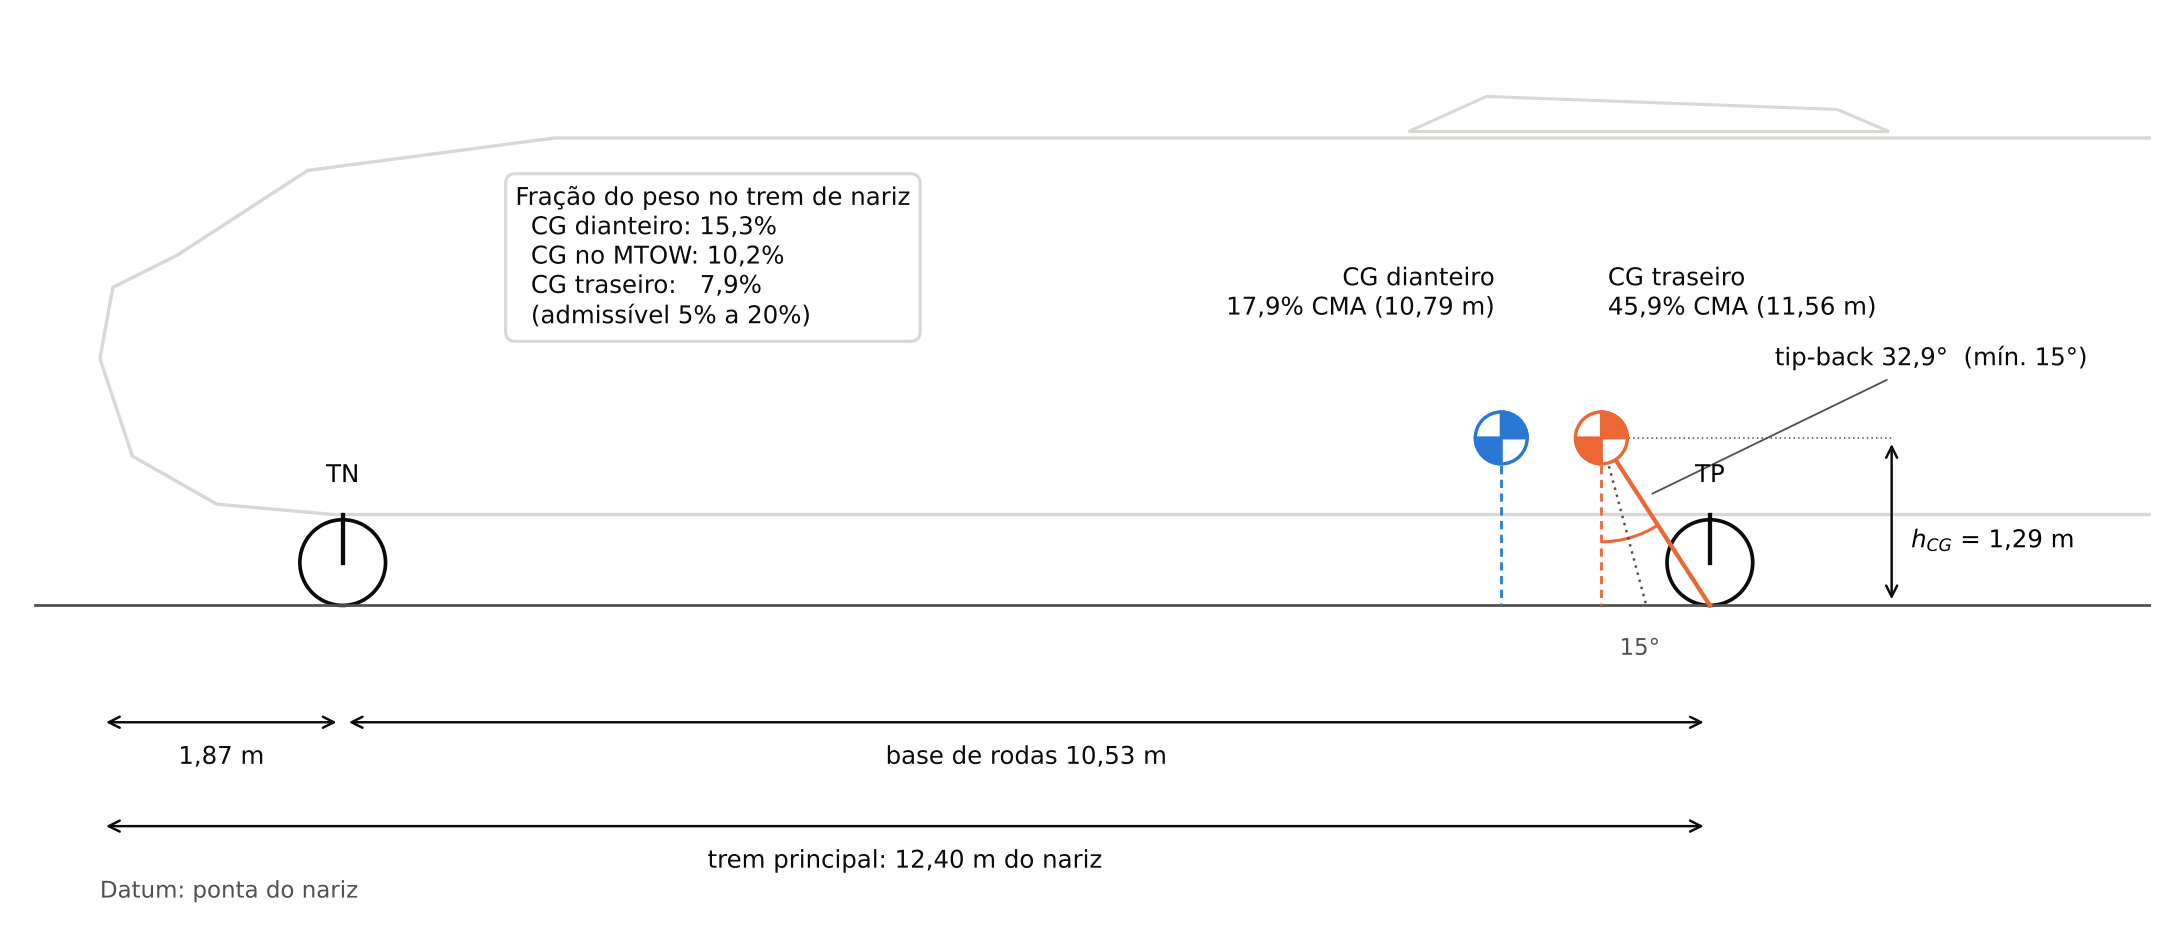
\includegraphics[width=\textwidth]{Images-CG/cg_trem_posicionamento.png}
\caption{Posicionamento longitudinal do trem de pouso em relação aos limites de CG.}
\label{fig:cg_trem}
\end{figure}

\begin{table}[H]
  \centering
  \linespread{1}\small
  \setlength{\tabcolsep}{4pt}
  \caption{Verificação do trem com o trem principal em 12,40 m e o trem de nariz em 1,87 m (cargas estáticas no MTOW).}
  \label{tab:cg_trem}
  \begin{tabularx}{\textwidth}{>{\raggedright\arraybackslash}X c c c c c c}
    \toprule
    \textbf{Condição} & $\bar{X}_{CG}$ \textbf{[m]} & $x_m$ \textbf{[m]} & $x_n$ \textbf{[m]} & \textbf{Tip-back} & \textbf{Nariz} & \textbf{Carga TP / TN [kgf]} \\
    \midrule
    Limite dianteiro (17,9\%) & 10,79 & 1,607 & 8,923 & 51,2° & 15,3\% & 19\,219 / 3\,461 \\
    CG no MTOW (37,3\%) & 11,33 & 1,074 & 9,456 & 39,8° & 10,2\% & 20\,368 / 2\,312 \\
    Limite traseiro (45,9\%) & 11,56 & 0,835 & 9,695 & 32,9° & 7,9\% & 20\,881 / 1\,799 \\
    \midrule
    \multicolumn{4}{l}{\textbf{Critério}} & $\geq 15^\circ$ & 5\% a 20\% & \\
    \bottomrule
  \end{tabularx}
\end{table}

Na Tabela~\ref{tab:cg_trem}, $x_m$ e $x_n$ são as distâncias horizontais do CG ao contato do trem principal e do trem de nariz, e as alturas são $z_m = z_n = 1{,}29$ m. Esses valores devem ser usados nas cargas de solo da Seção~\ref{sec:cargas_solo}. Para o dimensionamento de pneus, a carga máxima do trem principal ocorre no limite traseiro (92,1\% do peso) e a do trem de nariz no limite dianteiro (15,3\%), e não na divisão de 90\%/10\% adotada anteriormente.

\textbf{Precisa deslocar o trem?} Sim. O trem principal vai de 10,87 m para 12,40 m, 1,53 m para trás. Nessa posição ele fica sob a região da longarina traseira da raiz da asa (raiz de 10,08 m a 13,78 m), o que permite fixá-lo na caverna reforçada de ligação asa--fuselagem. O alojamento nas carenagens laterais deve ser redesenhado para essa estação.

\section{Valores de Entrada para os Demais Capítulos}
\label{sec:cg_saidas}

\begin{table}[H]
  \centering
  \linespread{1}\small
  \setlength{\tabcolsep}{4pt}
  \caption{Entradas de peso e CG a serem usadas em todo o relatório.}
  \label{tab:cg_entradas}
  \begin{tabularx}{\textwidth}{>{\raggedright\arraybackslash}X >{\raggedright\arraybackslash}X >{\raggedright\arraybackslash}X}
    \toprule
    \textbf{Grandeza} & \textbf{Valor} & \textbf{Usado em} \\
    \midrule
    MTOW & 22\,680 kgf (50\,000 lb) & Desempenho, Cargas, Estrutural, Estabilidade \\
    MLW & 22\,350 kgf & Desempenho (pouso), Cargas de solo \\
    MZFW & 19\,592 kgf & Estrutural (asa), Cargas \\
    OEW / peso vazio $W_E$ & 13\,512 / 13\,064 kgf & Desempenho (curva de pesos), resumo técnico \\
    Combustível com carga paga máxima / máximo & 3\,088 / 4\,990 kgf & Desempenho (alcance) \\
    Carga paga máxima & 6\,080 kgf & Desempenho, resumo técnico \\
    $X_{BA,\text{CMA}}$, $\bar{c}$ & 10,30 m; 2,755 m & Estabilidade, desenhos, Estrutural (apoios da fuselagem) \\
    Limites de CG & 17,9\% a 45,9\% da CMA (10,79 a 11,56 m) & Estabilidade, Cargas (casos dianteiro/traseiro) \\
    CG no MTOW & 11,33 m (37,3\% da CMA) & Cargas, Estabilidade \\
    Altura do CG ao solo & 1,29 m & Cargas de solo, trem \\
    Trem principal / de nariz & 12,40 m / 1,87 m & Desenhos, Cargas de solo, pneus \\
    Fração máxima no trem principal / de nariz & 92,1\% / 15,3\% & Pneus e freios \\
    \bottomrule
  \end{tabularx}
\end{table}

\section{Limitações}
\label{sec:cg_pendencias}

Os braços dos sistemas distribuídos e da fuselagem são os que mais pesam no resultado. Um metro de erro no braço do mobiliário desloca o CG do peso vazio em 0,12 m (4,4\% da CMA), e no braço da fuselagem em 0,28 m (10,3\% da CMA). Em uma revisão futura, esses braços devem ser substituídos pelos centroides das massas obtidas no dimensionamento estrutural (Capítulo de Dimensionamento Estrutural), e os pesos estatísticos devem ser comparados com essas massas.

O braço dos comandos de voo (1,62 m) representa o conjunto inteiro no posto de pilotagem. Como a correlação de Roskam inclui cabos, atuadores e articulações até as superfícies, esse braço é conservador para o limite dianteiro.